\chapter{讲故事}
\section{相变模型:人脑、森林大火与冰的熔化}
啊。。一上来就要讲一个扯蛋的问题:人的意识是从哪里来的?

有一种理论认为人脑工作在临界状态,就像冰熔化成水的时候一样。我们把冰的熔点叫做一个临界点,温度离临界点远的地方全是水或者全是冰,而在临界点附近一部分是水,一部分是冰,并且冰和水的比例可以随着系统从外界吸收的热量而迅速调整。

人脑的行为也是类似的。人脑里有许多神经元,每个神经元可以处于静息或者兴奋状态,如果神经元全部静息或者全都一直兴奋,那就太没意思了;只有神经元一部分静息,一部分兴奋,才能传递信息。

我们可以对神经元建立一个简单的数学模型:

1、每个神经元与其他$n$个神经元相连,一个神经元兴奋之后可以让相连的神经元兴奋。我们把$n$叫作配位数,跟晶体的说法一样。这个过程有一段延迟时间$\tau$,但是接下来我们会发现,它对我们要研究的问题并不重要,因为其他东西都没有时间的量纲。

2、一个神经元兴奋之后有一定概率$k$深藏功与名,不让相连的神经元兴奋。这个过程在生物学上的原理我们就不去深究了,这只是一个数学模型。我们把$k$叫作耗散强度。

配位数和耗散强度这两个参数可以描述人脑的行为。如果配位数很小,耗散强度很大,兴奋就会很快停止传播;如果配位数很大,耗散强度很小,兴奋很容易传了一圈又回来,造成神经元一直兴奋,这两种情况都是我们不希望看到的。只有配位数和耗散强度合适,神经元才能一会兴奋一会静息,这时候我们说人脑达到了一种临界状态。

这个数学模型在许多实际问题中都会出现。比如森林着火的时候,一棵树有一定概率$(1-k)$点燃周围的$n$棵树。如果配位数很小,耗散强度很大,火就会很快熄灭;如果配位数很大,耗散强度很小,整片森林就会很快烧完;只有配位数和耗散强度合适,火才能烧很长时间。

但是人脑和森林有一个区别:人脑当中一个神经元兴奋一次之后可以再兴奋,而森林中一棵树烧掉了就不能烧第二次。事实上,这个区别并不重要。我们可以在森林中画出一块边长为$l$的区域,然后研究这块区域烧完需要的时间$t$。(区域的大小这里用边长而不用面积表示,而且区域是正方形、三角形还是圆形之类的也不重要)

最简单的研究方法就是用电脑来模拟这个数学模型。可以发现,$t$与$l^{\alpha}$成正比,$\alpha$是一个由配位数和耗散强度决定的参数。另外,$t$显然与一棵树烧完需要的时间$\tau$成正比。于是,怎么用$n$和$k$算出$\alpha$成为了最重要的问题,除了计算机模拟,科学家们正在想办法找出数学上的表达式。

一个区域的面积与$l^2$成正比,因为面积是二维的。事实上,$\alpha$也是一种相当于维度的东西,但是它不一定是整数。

我们联想到数学上的分形图案,你可能听说过,它们也有分数的维度。这里的维度是怎么定义的呢?比如一个正方形,把它的边长扩大到原来的$2$倍,相当于把$4$个原来的正方形拼起来,所以它的维度是$\log_2 4=2$。而图\ref{fig-sierpinski}是著名的Sierpinski三角,把它的边长扩大到原来的$2$倍,相当于把$3$个原来的图形拼起来,所以它的维度是$\log_2 3=1.585 \dots$而在森林大火的例子中,如果区域的边长扩大到原来的$2$倍,那么这块区域烧完需要的时间$t$就会扩大到$2^{\alpha}$倍。
\begin{figure}[htb]
\centering
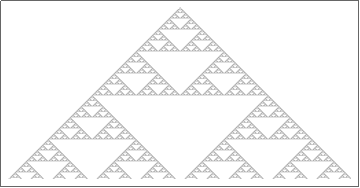
\includegraphics[scale=1]{fig/sierpinski.png}
\caption{传说中的Sierpinski三角}
\label{fig-sierpinski}
\end{figure}

(博哥在我们班上课的时候曾经说过“多尺度是现在热门的研究方向”)(顺便说一句,除了相变,物理学中的另一个热门问题——湍流,也与分形有关)(啊。。好像扯远了)

接下来举一个看起来比较像物理的例子:磁铁。我们可以认为磁铁里面有许多磁铁分子(虽然严格来说不叫分子),它们喜欢通过异极相吸来整齐地排列在一起,如图\ref{fig-magnet-mole},而且排列得越整齐,异极相吸的作用就越强,这里每个分子附近的分子数量就是配位数。同时,这些分子会做热运动,破坏这种整齐的结构,这里热运动的强度就是耗散强度。
\begin{figure}[htb]
\centering
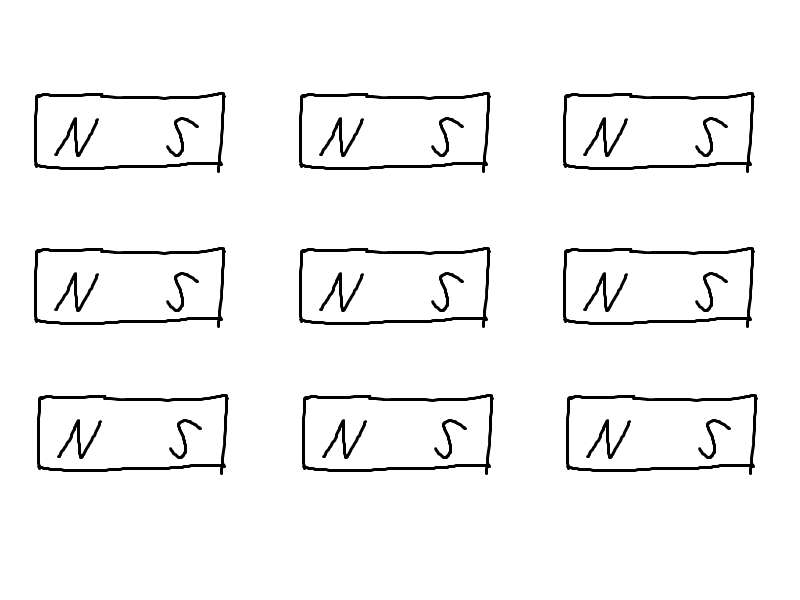
\includegraphics[scale=0.5]{fig/magnet-mole.png}
\caption{啊,乖乖站好}
\label{fig-magnet-mole}
\end{figure}

配位数是由磁铁的物质结构决定的,而耗散强度由温度决定。如果温度很低,磁铁就有磁性;如果温度很高,磁铁就会失去磁性;如果温度达到某个临界点,磁铁的磁性就会明显受外界扰动的影响。

现在终于可以讲冰熔化的过程了。水分子之间也有一种作用力来让它们排列整齐,你可能会想到偶极力,但是并没有这么简单,与水分子的米老鼠形状有关。(下次讲故事会讲到)而水分子的耗散仍然是热运动。在临界点附近,水分子的整齐程度也会明显受外界扰动的影响。

另外,这几个模型都有一个共同点:每个神经元、每棵树、每个磁铁分子都遵循很简单的规律,但是合起来就会出现复杂的现象。这种系统称为\emph{元胞自动机},比如康威的生命游戏就是一个著名的例子。
\section{马尔可夫链:语感与概率}
然后又要讲一个扯蛋的问题:我们做语文用的“语感”到底是什么?
\section{关于非线性化学反应}
博哥在上课的时候说化学反应是非线性的,所以初始反应物浓度越高,全部反应所需的时间越短。当时我说非线性的意思是反应速率不但与反应物的浓度有关,还与速率有关,但是“速率与速率有关”这句话是经不起推敲的。

简单起见,考虑只有一种反应物的情况。如果反应速率只与浓度有关,可以表示为$\frac{\opd n}{\opd t}=-A n$,$A$是比例系数。

如果反应速率与浓度和速率有关,就变成$\frac{\opd n}{\opd t}=-A n-B \frac{\opd n}{\opd t}$,也就是$\frac{\opd n}{\opd t}=-\frac{A}{1+B} n$。

如果考虑浓度对时间的二阶导,则变成$\frac{\opd^2 n}{\opd t^2}=-A n-B \frac{\opd n}{\opd t}$,但是这仍然是一个线性的方程。

非线性项可以是浓度与速率的乘积,比如$\frac{\opd^2 n}{\opd t^2}=-A n-B \frac{\opd n}{\opd t}+C n \frac{\opd n}{\opd t}$,结果如图\ref{fig-nonlinear-reaction}
\begin{figure}[htb]
\centering
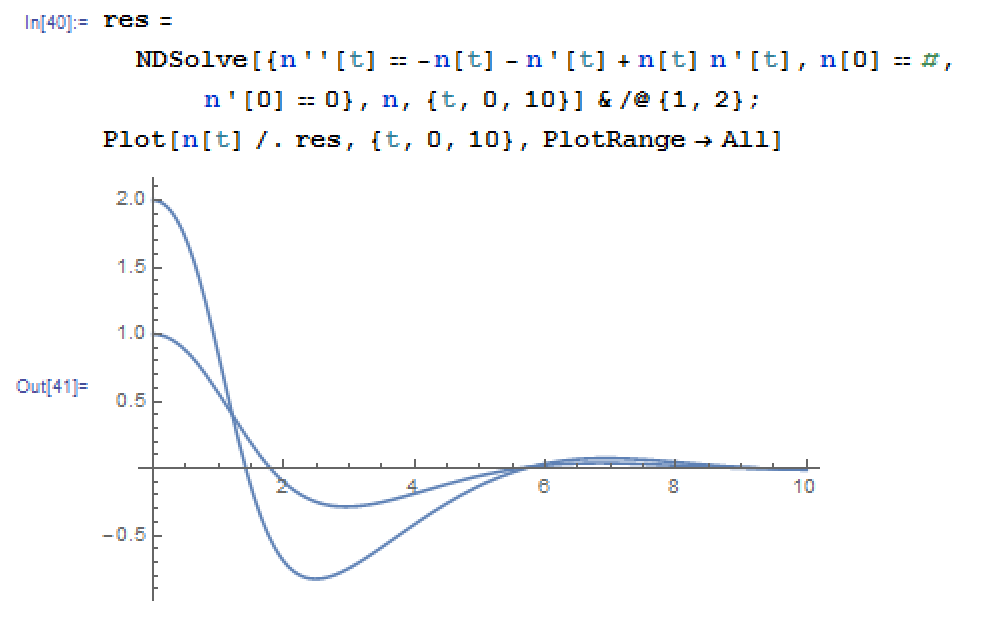
\includegraphics[scale=0.5]{fig/nonlinear-reaction.png}
\caption{但是一不小心浓度就会小于0}
\label{fig-nonlinear-reaction}
\end{figure}

另一种把方程搞成非线性的方法是引入时间关联,比如$\frac{\opd n(t)}{\opd t}=-A n(t)-B n(t-t_1)$,$t_1$是一个常量,表示当前时刻和$t_1$之前的那个时刻的浓度都对当前时刻的速率有影响。
